\chapter{Results}
\label{cha:result}




\section{Direct Cost}\
\label{sec:direct_cost}

Here is the example to show how to include a figure. Figure~\ref{fig:cost}
includes two subfigures (Figure~\ref{fig:zerocost}, and Figure~\ref{fig:zerobus});

\begin{figure*}
  \label{fig:cost}
  \subfigure[Fraction of cycles spent on zeroing\label{fig:zerocost}]{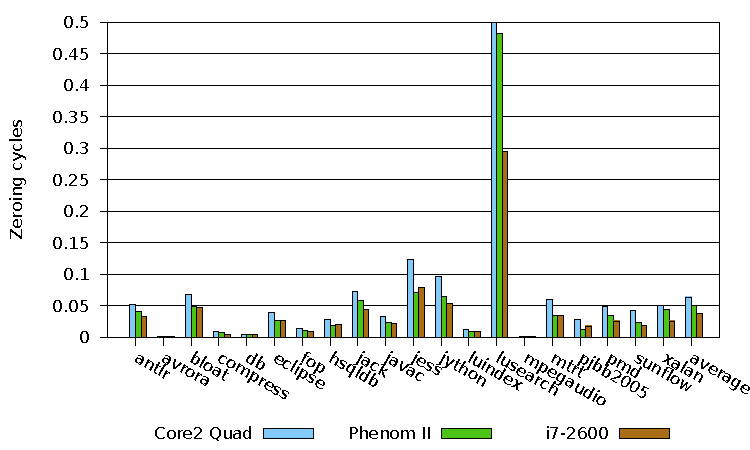
\includegraphics[width=\columnwidth]{figs/zerocost_intel.pdf}}
  \subfigure[BytesZeroed / BytesBurstTransactionsTransferred\label{fig:zerobus}]{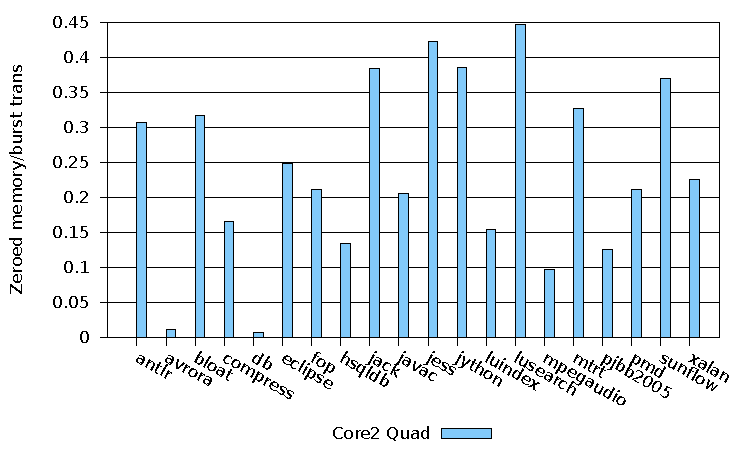
\includegraphics[width=1.0\columnwidth]{figs/zerobus_core.pdf}}
  \caption{The cost of zero initialization}
\end{figure*}


\begin{figure}
  \centering
  \subfigure[\label{fig:c:hello}]{
  \begin{minipage}[b]{\columnwidth}
    \lstinputlisting[linewidth=\columnwidth,breaklines=true]{code/hello.c}\vspace*{-2ex}
  \end{minipage}}
  \subfigure[\label{fig:java:hello}]{
  \begin{minipage}[b]{\columnwidth}
    \lstinputlisting[linewidth=\columnwidth,breaklines=true]{code/hello.java}\vspace*{-2ex}
  \end{minipage}}
  \caption{Hello world in Java and C.}
  \label{fig:helloworld}
\end{figure}

\section{Summary}
